\chapter{The torus topology}
\label{ch:torus}

\section{What changes}
A $4\times4$ torus joins the opposite edges of the mesh with eight extra links, so every core has four neighbours and the longest path shrinks from six hops to four. Everything else is held as in the
mesh experiments: the same ten benchmarks, the same mapper (HQA) with the same seeds, the same ACE parameters, the same link length for every link (a folded layout; the wrap links are not longer),
the same scheduler, budgets, policies, physics seeds and controls.

\paragraph{Routing.} The routes are the mapper's own: a Dijkstra search for the path with the fewest hops, with the product of link reliabilities as the tie-break (route model \code{shortest}), exactly as for the mesh
traces. The mapping-only path of the study script was checked to reproduce the archived mesh trace line for line before it was used for the torus. ACE itself needed three changes: trace validation
knows wrap-around links; the topology file is generated from the mesh file by adding the eight wrap links in the mesh's own link format (every router then has four quantum links, tested by loading it in ACE);
and a torus trace is refused on a mesh topology file and the reverse.

\paragraph{One caveat.} The mapper is run on the torus graph, so the torus traces differ from the mesh traces in the placement as well as the routes. Differences below are differences of the two systems, not of the topology alone.

\section{Results}
Torus traces need 11\% to 37\% fewer hops than the mesh traces (CDKM 11\%, QFT 23\%, QAOA 16\%, GHZ 25\%, VQE 37\%). Every control passed on all 1\,368 runs, as for the mesh (Chapter~\ref{ch:exp1}).
\begin{table}[H]
\centering\small
\begin{tabular}{@{}lrrrrr@{}}
\toprule
Workload & Hops & Overload\% at C=4 & On-demand ms, 2 mem. & On-demand ms, 4 mem. & Dynamic ms, 8 mem. \\
\midrule
GHZ & 24/18 & 0.0/0.0 & 1.17/1.15 & 1.17/1.15 & 0.26/0.28 \\
Bernstein--Vazirani & 25/21 & 0.0/0.0 & 1.22/1.11 & 1.22/1.11 & 0.24/0.23 \\
BMW/QUARK cardinality & 144/108 & 0.0/0.0 & 1.12/1.10 & 1.12/1.10 & 0.25/0.25 \\
VQE real amplitudes & 104/66 & 6.1/1.5 & 1.11/1.14 & 1.11/1.14 & 0.25/0.30 \\
CDKM ripple-carry adder & 456/406 & 0.6/0.6 & 1.24/1.11 & 1.14/1.09 & 0.30/0.29 \\
Graph state & 76/60 & 33.3/38.9 & 2.72/1.86 & 1.24/1.11 & 0.95/0.62 \\
Draper QFT adder & 1310/984 & 41.3/25.8 & 2.16/2.25 & 1.15/1.13 & 0.89/0.74 \\
QAOA & 3068/2562 & 71.6/57.9 & 3.42/2.47 & 1.27/1.17 & 1.86/1.10 \\
QFT & 2510/1938 & 65.2/58.0 & 4.72/2.79 & 1.59/1.21 & 2.78/1.16 \\
Random circuit & 11688/9574 & 8.0/3.4 & 1.27/1.19 & 1.11/1.11 & 0.38/0.29 \\
\bottomrule
\end{tabular}
\caption{Mesh/torus. Hops: mean requests per trace. Overload: \% of active layers with any core above capacity 4. Latencies are means over nine runs.}
\label{tab:torus}
\end{table}

On-demand latency under congestion improves: at two memories QFT goes from $4.72$ to $2.79$\,ms, QAOA from $3.42$ to $2.47$\,ms and graph state from $2.72$ to $1.86$\,ms; at four memories QFT from $1.59$ to $1.21$\,ms. Dynamic pre-generation also gets faster under congestion (QFT at eight memories: $2.78$ to $1.16$\,ms). The structural overload at capacity four falls for most workloads (QFT 65.2\% to 58.0\%, QAOA 71.6\% to 57.9\%, Draper 41.3\% to 25.8\%) but not for graph state, where
it rises from 33.3\% to 38.9\% (only six layers are active, so a single layer is 17 percentage points). Draper at two memories is slightly slower on the torus ($2.16$ to $2.25$\,ms).

\clearpage\newgeometry{margin=12mm}\begin{landscape}
\begin{figure}[p]
\centering
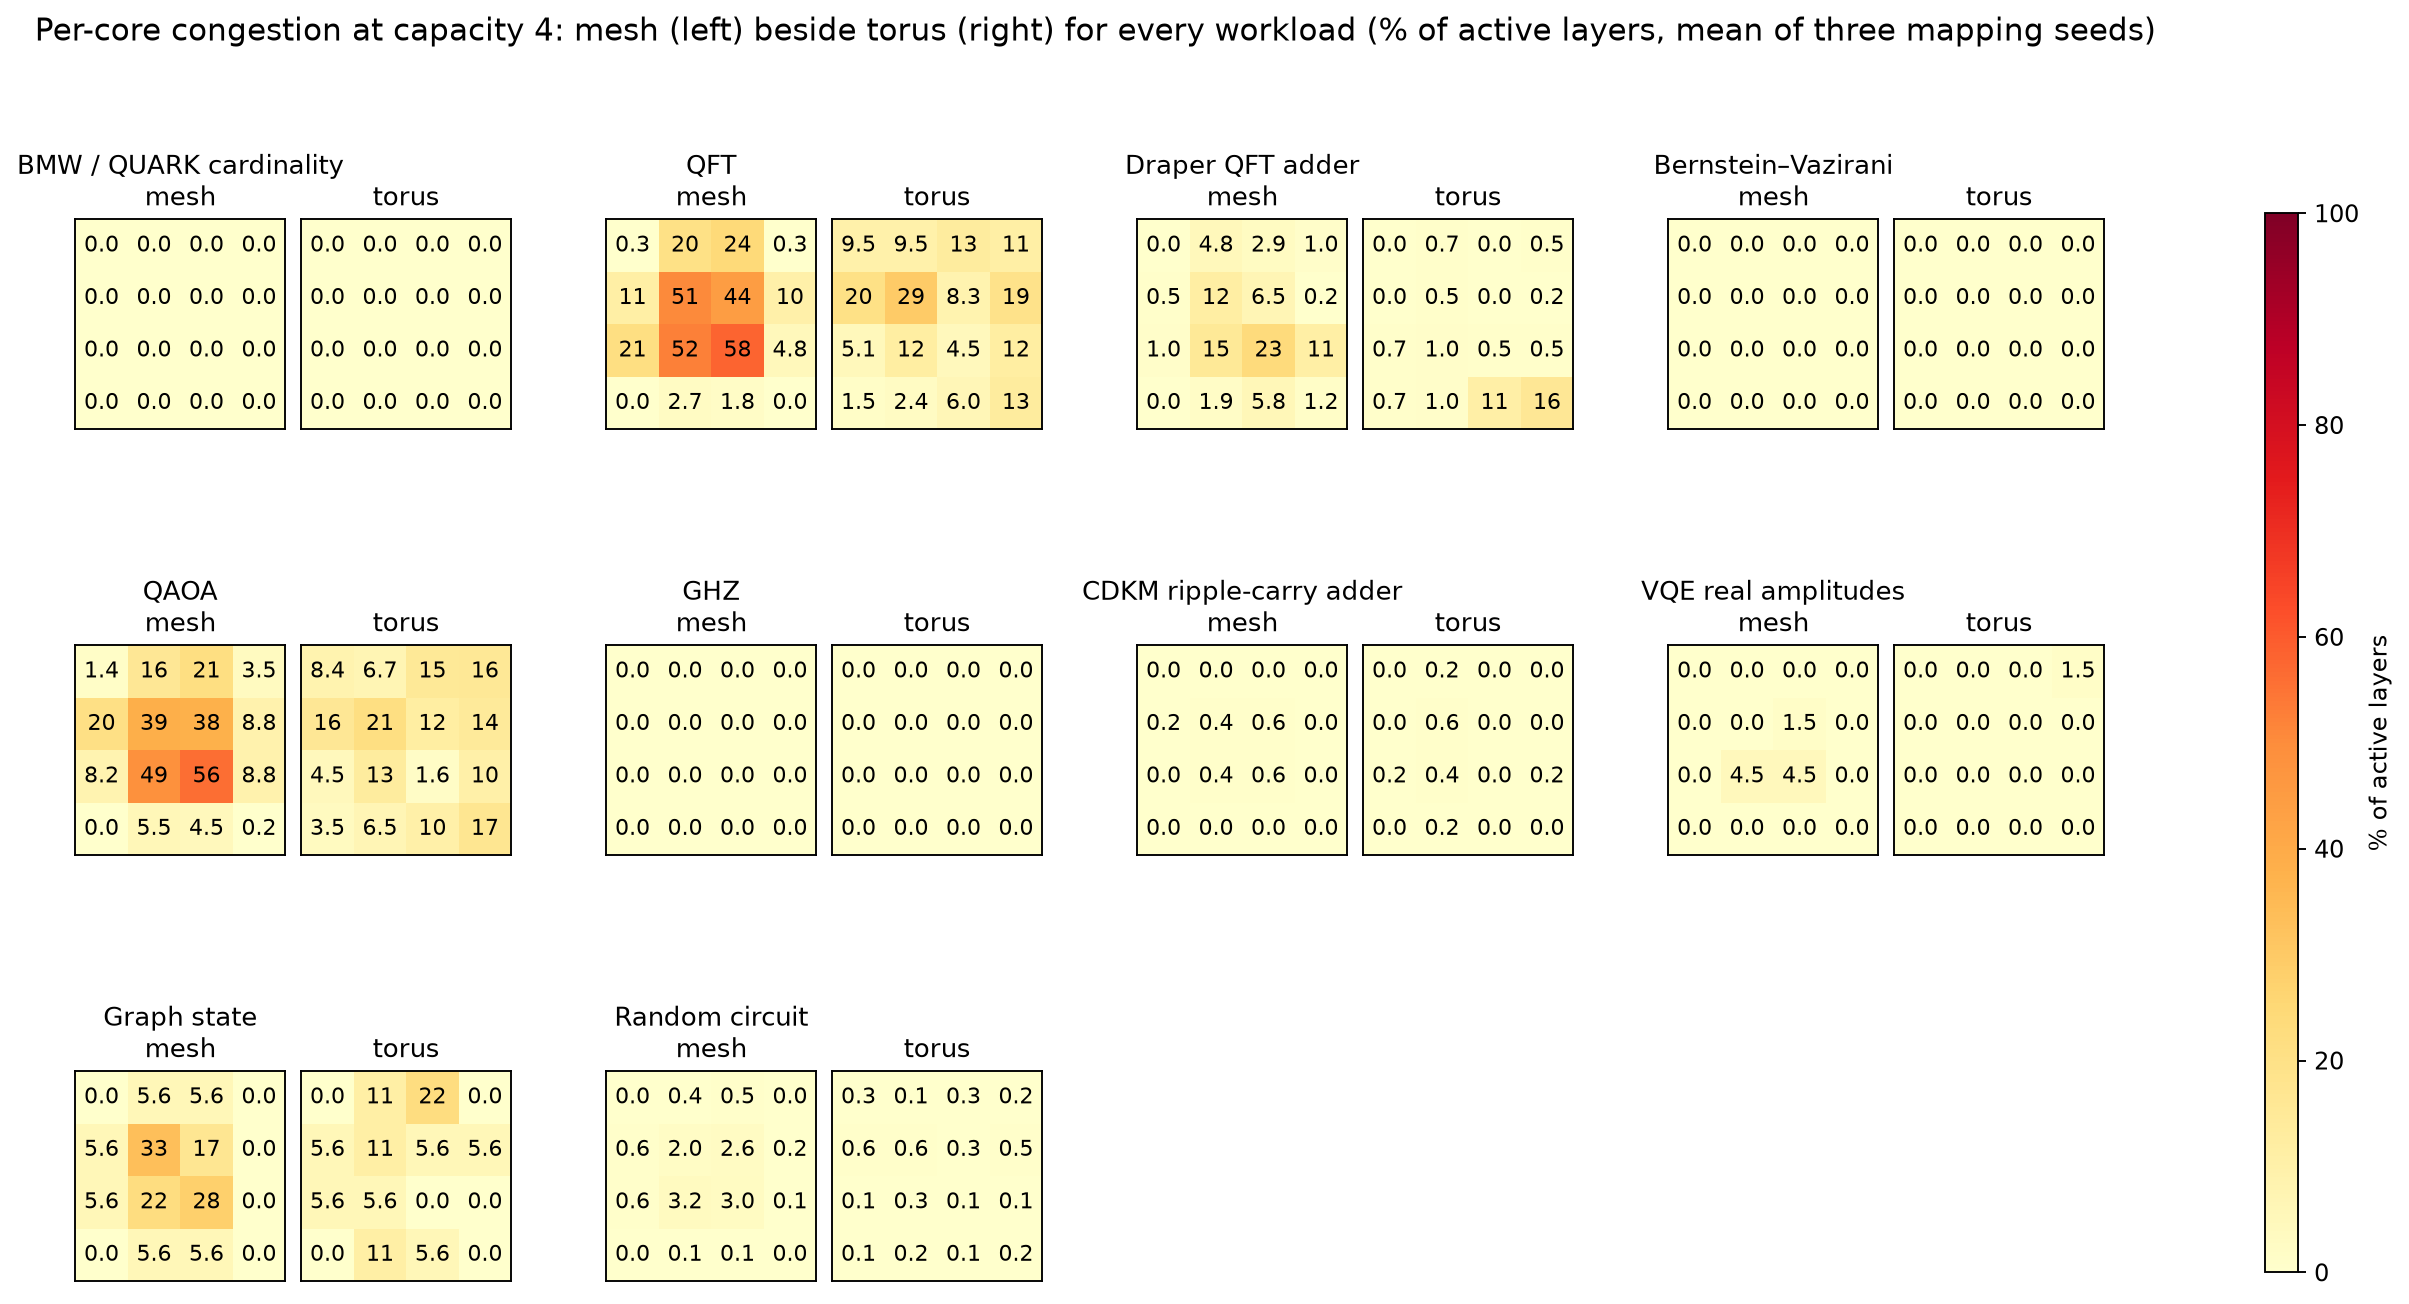
\includegraphics[width=\linewidth,height=0.82\textheight,keepaspectratio]{mesh_vs_torus_heatmaps.png}
\caption{Per-core congestion at capacity 4 on the mesh (left of each pair) and on the torus (right), for every workload. The torus lowers the overload in five workloads, leaves four unchanged and raises it for graph state; the traces differ in placement as well as topology.}
\label{fig:mesh-vs-torus}
\end{figure}
\end{landscape}\clearpage\restoregeometry

